\chapter{Dostupné testovací nástroje}
V kapitole dostupné testovací nástroje budou zkoumána část dostupných opensource i komerčních nástrojů pro všechny fáze testování. U všech nástrojů bude posuzován přínos v případě nasazení v testovacím systému pro výrobky společnosti Conel.

\section{Jenkins CI}
Jenkins CI je nástroj pro kontinuální integraci. Kontinuální integrace spočívá v častém kompilování zdrojového kódu a následném spouštění testů nad tímto softwarem.
Jenkins je prográm napsaný v programovacím jazyce Java. Tento nástroj umí podoru kompilace různých projektů podporu pluginů jejichž počet neustále roste.

\begin{figure}[h]
  \centering
  
\includegraphics[width=.3\LW]{jenkins_logo}
  \caption{Logo produktu http://www.jenkins-ci.org}
  \label{fig:testlink_logo}
\end{figure}

Jenkinsen je dobrý a přehledný buildovací systém s podporou mnoha programovacích jazyků. Velikou výhodou tohoto systému je opensource řešení tohoto projektu. Naopak nevýhodou jsou veliké systémové požadavky tohoto nástroje. Další nevýhodou je že tento systém podporuje testování, ale podporuje pouze testování na úrovní testování jednotek, které v navrhovaném systému nebude vůbec použito. Naopak funkční a systémové testování na konkrétním hardwaru.

\begin{figure}[h]
  \centering
  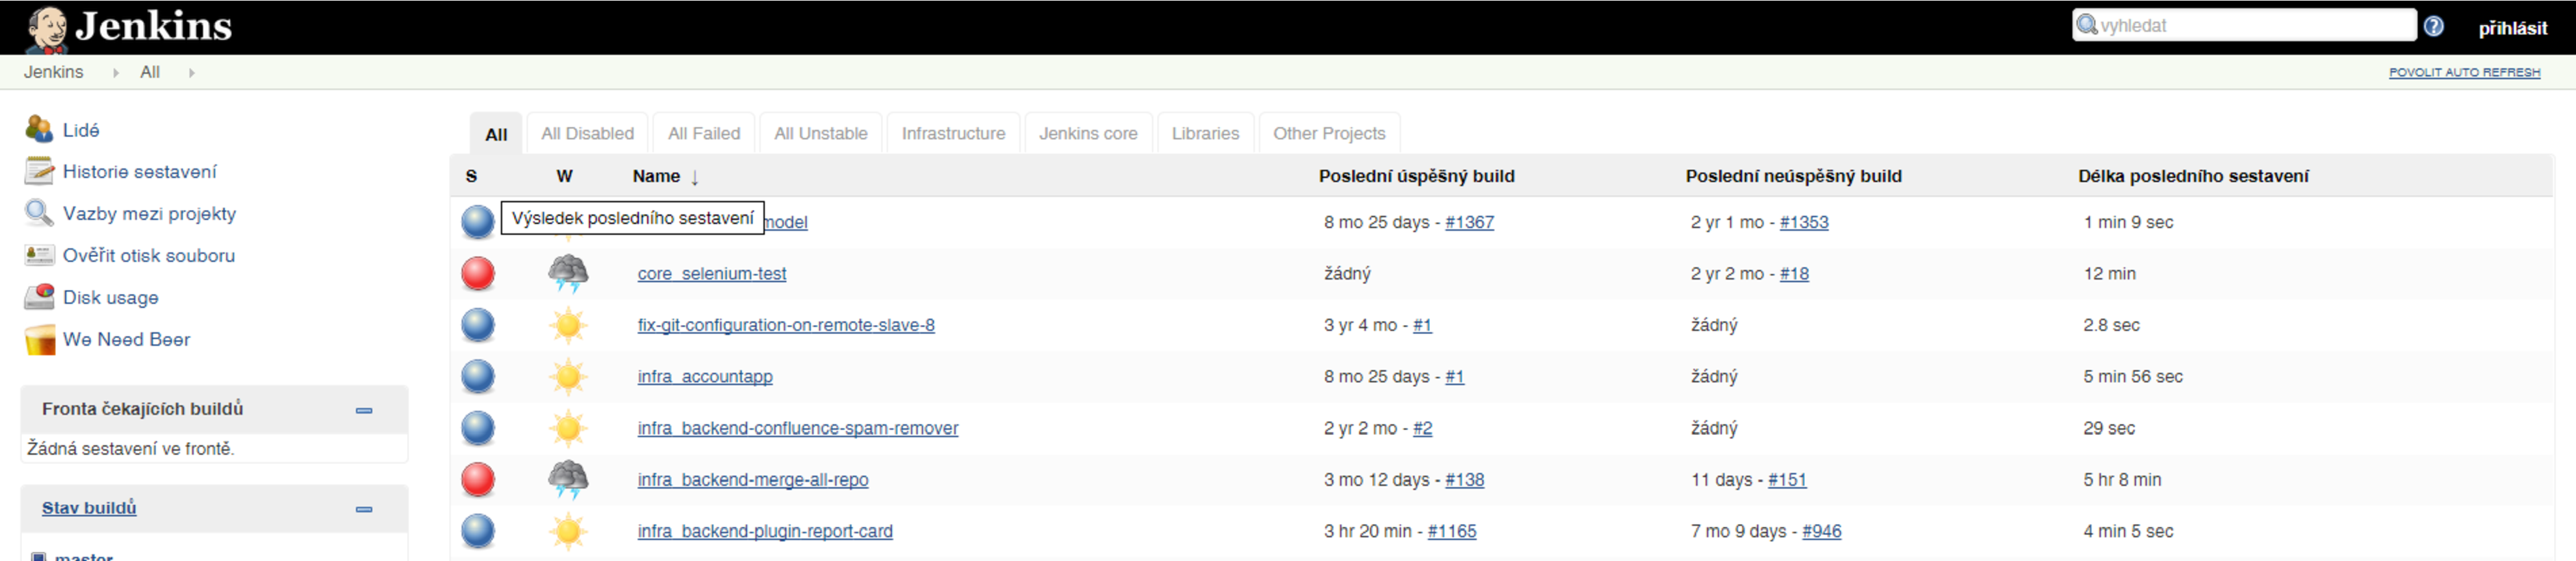
\includegraphics[width=\LW]{jenkins_example}
  \caption{Příklad otevřené aplikace Jenkinsen}
  \label{fig:testlink_example}
\end{figure}

Použití tohoto nástroje pro konitunální integraci v testovacím zařízení by bylo možné pouze ve fázi buildování všech firmwarů. Jelikož skripty zajišťující správnou funkci s buildovacím program ltib, který je používán pro překlad většiny výrobků, je potřeba napsat stejné jak při použití Jenkinse tak při vlastním spouštění buildů, budou muset být napsány stejné. Taktéž pro spouštění skriptů pro překlad je totožné se spouštěním skriptů pro testování. Na zákldě těchto skutečností jsem upřednostnil použití vlastního spouštění testů, hlavně z důvodu jednotného systému pro vizualizaci všech informací o průběhu célé fáze testování.

\section{Testlink}
Testlink je nástroj pro správu a organizaci testů. Nástroj je dělaný jako webová aplikace napsaná v jazyce PHP a využívající databázi MySQL nebo PostgeSQL. Aplikace je zdarama i pro komerční účely, jelikož je šiřiné pod licencí GPL.

\begin{figure}[h]
  \centering
  
\includegraphics[width=.3\LW]{testlink_logo}
  \caption{Logo produktu http://www.testlink.org}
  \label{fig:testlink_logo}
\end{figure}

Nástroj testlink umí dobře spravovat a organizovat testy a testovací případy. Nástroj obsahuje pět základních pilířů o které se dále opírá a tvoří jeho strukturu. Prvním a základním prvkem je testovací případ neboli test case. Tato položka odpovídá již odpovídajícímu testovacímu skriptu či testovací proceduře popisované ve způsobech testování. Dalším prvkem je sada testů označovaná test suite. Sada testů organizuje testy do funkčních skupin. Třetím prvkem nástroje testlink je testovací plán. Testovací plán je sestaven ze sad testů a dále z informací o daném testování. Dalším prvkem je testovací projekt, který je základním prvkem. Testovací projekt v známé terminologii odpovéda testovanému subjektu. Posledním prvkem tohoto systému je uživatel. Jednotlivý uživatelé maji různá práva úprav v systému, aby byla zavedena bezpečnost systému. Tento systém umí dále podle vložených výsledků testů vytvářet reporty o testování v různých formátech.

\begin{figure}[h]
  \centering
  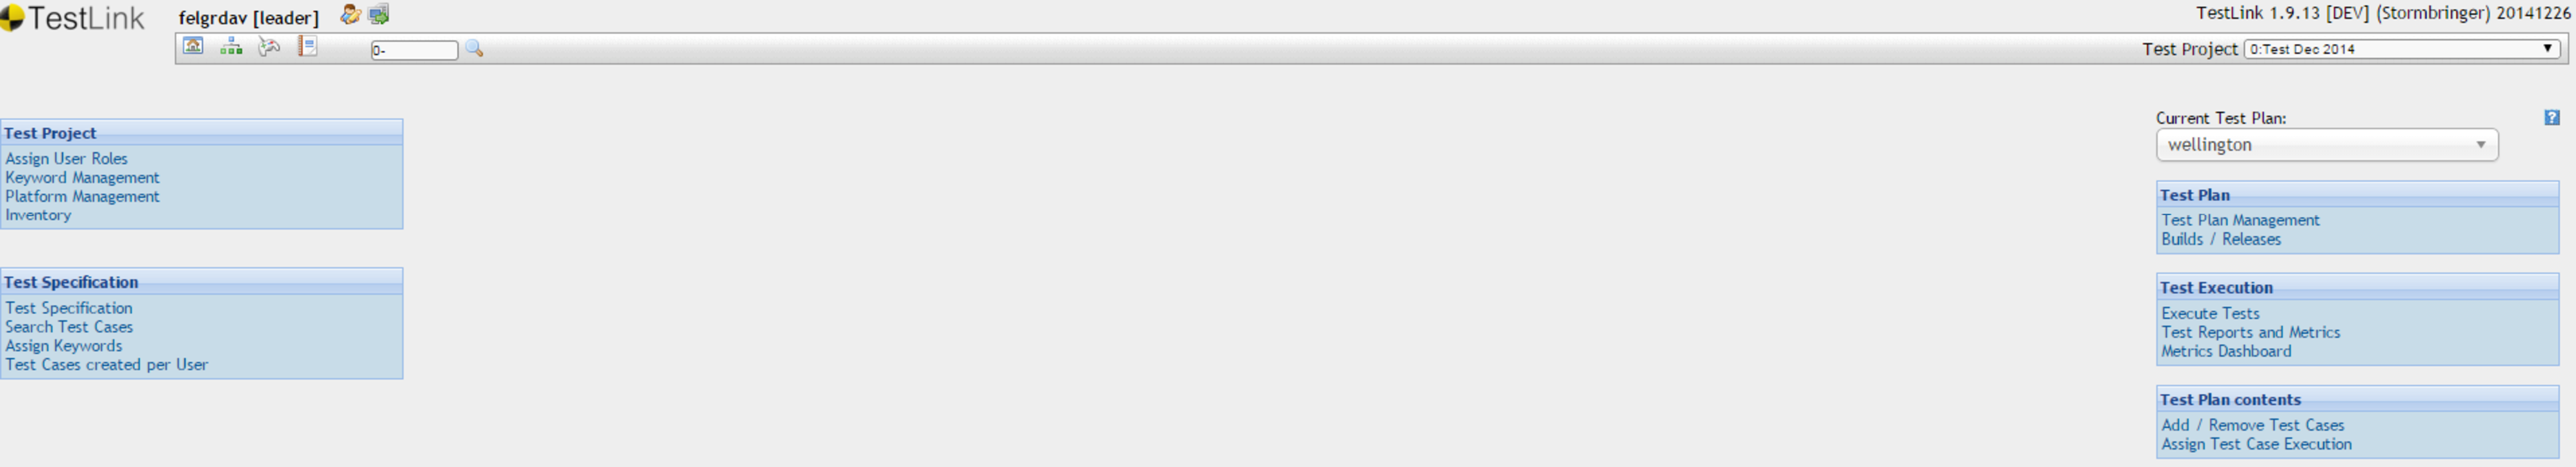
\includegraphics[width=\LW]{testlink_example}
  \caption{Příklad otevřené aplikace Testlink}
  \label{fig:testlink_example}
\end{figure}

Nástroj Testlink může být účiný v případě manuálního testování pro snadnou správu testů a reportování výsledků těchto testů. I v případě testovacího systému společnosti Conel by bylo možné systém nasadit, s tím že byly nutné úpravy tohoto systém k nasšim požadavkům automatického testování a speciálním požadavkům na modulárnost testovaných výrobků. Po krátkém zkoumání jsem zjistil že úpravy pro automatické testování a úpravy k potřebám hiearchie testovací laboratoře by byli rozsáhlé. Dále tento systém působí velmi nepřehledně. Díky těmto závěrům bylo rozhodnuto nepoužití tohoto nástroje pro spravování testů a reportování výsledků.


\section{Selenium}
Selenium je nástroj pro testování webových aplikací. Tento nástroj je také opensource program napsaný v jazyce Java. Selenium je dostupné ve čtyřech variantách a to Selenium IDE, Selenium RC, Selenium WebDriver a Selenium Grid. Selenium IDE je plugin do internetového prohlížeče Firefox. Dále Selenium RC, který si sám pouští internetové prohlížeče a provádí na nich testy. Testy je možné psát v Java, C, Python, Ruby, Perl, PHP a je pro psaní těchto testů připraveno přehledné API. Sleneium WebDriver usndňuje psaní samotných testů na úkor nutnosti psaní všech testů na každý prohlížeč. Poslední Selenium Grid umožňuje paralérní spouštění testů na více strojch i počítačích.

\begin{figure}[h]
  \centering
  
\includegraphics[width=.1\LW]{selenium_logo}
  \caption{Logo produktu http://www.seleniumhq.org}
  \label{fig:selenium_logo}
\end{figure}

Selenium je dobrý nástroj pro testování webových aplikací. Určitě využitelný i pro testování samotných routerů. Bohužel v první fázi budou jednotlivé konfigurace měněni pomocí ssh a telnet přístupu do routeru a jelikož tento nástroj více možností neobsahuje, tak nebude v první fázi nasazování testovacího zařízení použit.

\section{VectorCAST}
Nejlepším zkoumaným nástrojem byl komerční produkt VectorCAST od společnosti VECTOR Software.



Podporuje celou škálu testování.
Nemožnost úpravy, komerční licence.



\section{Embedded Unit}
Vhodné pro embedded systémy.
Podporuje pouze UNIT testy.



\section{GNU/Linux Desktop Testing Project}
Testování Linuxových grafický prostředí.

\section{Linux Test Project}
Testování Linuxového jádra.
Možné budoucí nasazení jako modulu.


\section{Maveryx}
Podporuje pouze JAVU.


\section{Robot Framework}
Dobrý testovací Framework.
Jednoduché dopisování testů pomcí Pythonu.
Nutné dopsat testovací syntaxi, testovací API, aplikační interface.


\section{The Software Testing Automation Framework (STAF)}
Nepodporuje systémová testování.






\endinput
